\documentclass[11pt, twoside]{report}

\usepackage{fontspec}
\usepackage[utf8]{inputenc}
\usepackage[bitstream-charter]{mathdesign}
\usepackage{bbding}
\usepackage{ragged2e}
\usepackage{parskip}
\usepackage{enumitem}
\usepackage{titlesec}
\usepackage{paracol}
\usepackage{mdframed}
\usepackage[margin=1in]{geometry}

\usepackage[autocompile]{gregoriotex}

\titleformat{\chapter}[block]{\huge\scshape\filcenter}{}{1em}{}
\titleformat{\section}[block]{\Large\bfseries\filcenter}{}{1em}{}

\mdfsetup{skipabove=\topskip, skipbelow=\topskip}

\newcommand{\rubric}[1]{
	\switchcolumn[0] {
		\itshape
		#1
	}
}

\newcommand{\latinenglish}[2]{
	\switchcolumn[0]* {
		#1
	}
	\switchcolumn[1] {
		\itshape\small
		#2
	}
}

\newcommand{\latinenglishequal}[2]{
	\switchcolumn[0]* {
		#1
	}
	\switchcolumn[1] {
		\itshape
		#2
	}
}

\newenvironment{latinenglishsection}
	{\columnratio{.7, .3} \begin{paracol}{2}}
	{\end{paracol}}

\newenvironment{latinenglishequalsection}
	{\columnratio{.5, .5}\begin{paracol}{2}}
	{\end{paracol}}

\setlength{\columnseprule}{0.4pt}

\newcommand{\heading}[1]{
	\begin{leftcolumn}
		#1
	\end{leftcolumn}
}

\newcommand{\spanning}[1]{
	\switchcolumn*[#1]
}

\newenvironment{verses}[1]
	{\begin{flushleft} \begin{enumerate}[leftmargin=*] \setcounter{enumi}{#1}}
	{\end{enumerate} \end{flushleft}}

\newenvironment{versicles}{\par\leavevmode\parskip=0pt}{}

\newenvironment{collect}
{
	\leavevmode
	\parindent=1em
	\parskip=0pt
	\noindent Orémus.\par
}{}

\newenvironment{optionbox}
{
	\switchcolumn[0]
	\begin{mdframed}
%	\begin{minipage}{0.8\linewidth}
}{
%	\end{minipage}
	\end{mdframed}
}

\newcommand{\optionrule}{
	\begin{center}
	\rule{0.5\linewidth}{0.6pt}
	\end{center}
}

\newenvironment{optionruled}
{
	\optionrule
}
{
	\optionrule
}

% for use inside the collect environment
\newcommand{\Amen}{\par\noindent \Rbar. Amen.}

\begin{document}

%\title{Compline of The Blessed Virgin Mary}
%\date{ }

\vspace*{2cm}

\begin{center}
	\textbf{\Huge Compline of the Blessed Virgin Mary}\\
	{\LARGE According to the Washtenaw Use}
\end{center}

\vspace*{1cm}
%\maketitle

%\begin{figure}[h!]
	%\centering
%\end{figure}

\begin{center}
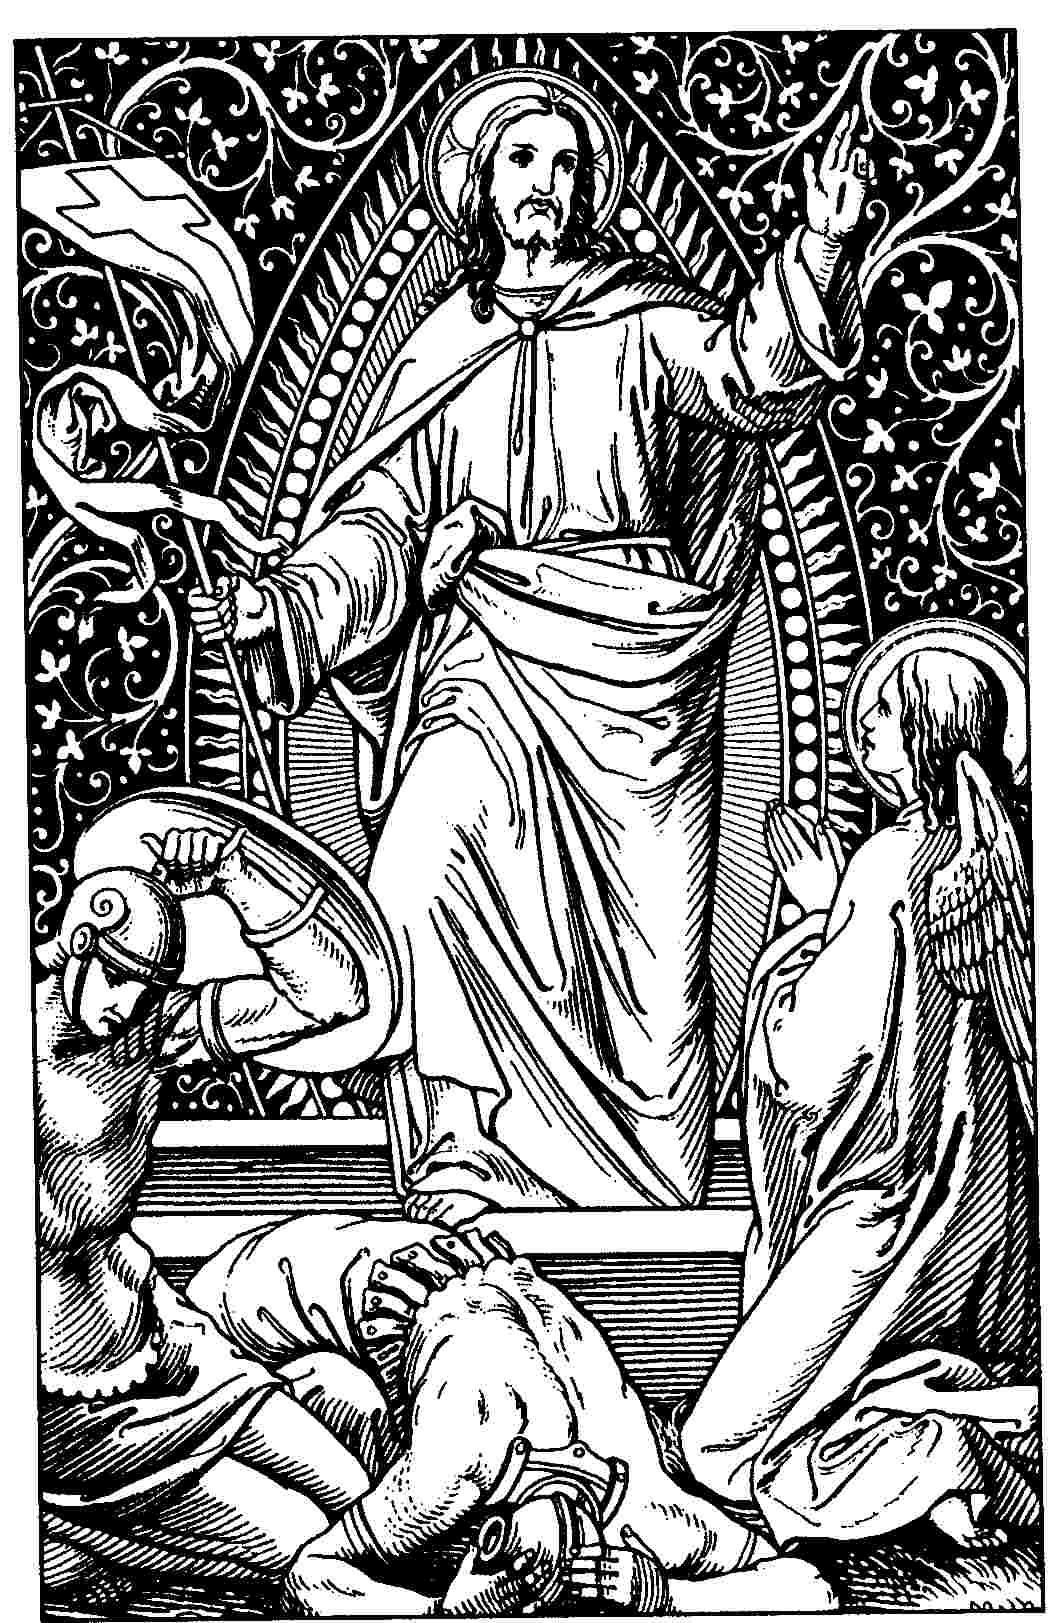
\includegraphics[width=0.6\textwidth]{ChristResurrected}
\end{center}

\hspace{0pt}
\vfill

\pagebreak

\vspace*{7.5cm}
``\textit{Compline} is the end of the day; and in the end of our life we have most need of Our Lady's help, and therefore, in all these Hours, we ought to do her veneration. Also, the pains that our Lord, Jesus Christ, suffered in His Holy Passion in all these seven hours, as is before said, Our Lady, His Mother, suffered the same pain in her hert by compassion, and therefore it is convenient to honor her and do her service in all the same hours.'' (Paraphrased from the \textit{Mirror of Our Lady}.) O most blessed Virgin, as the day draws to a close, may your prayers be ever with us. Amen.
\vfill

\pagebreak

\chapter*{Before Compline}

\section*{Preparatory Prayers}

\textit{ All kneel and pray silently. As you say the prayer \textnormal{Aperi, Domine}, make the sign of the cross with your thumb first over your lips, and then over your heart.}

\begin{latinenglishequalsection}

\latinenglishequal{
	Áperi, {\color{red}\maltese}\ Dómine, os meum ad benedicéndum\linebreak nomen sanctum tuum:
	{\color{red}\maltese}\ munda quoque cor meum ab ómnibus vanis, pervérsis et aliénis cogitatiónibus;
	intelléctum illúmina, afféctum inflámma, ut digne, atténte ac devóte hoc Offícium beátæ Vírginis Maríæ recitáre váleam,
	et exaudíri mérear ante conspéctum divínæ Majestátis tuæ.
	Per Christum Dóminum nostrum. 
	Amen.
}{
	Open, {\color{red}\maltese}\ O Lord, my mouth to bless Thy holy Name; {\color{red}\maltese}\ cleanse also my heart from all vain, evil, and wandering thoughts; enlighten my understanding and kindle my affections; that I may worthily, attentively, and devoutly say this Office of the Blessed Virgin Mary, and so merit to be heard before the presence of Thy divine Majesty.  Through Christ our Lord.  Amen.
}

\latinenglishequal{
	Domine, in unióne illíus divínæ intentiónis, qua ipse in terris laudes Deo persolvísti, has tibi Horas persólvo.
}{
	O Lord, in union with that divine intention wherewith thou, whilst here on earth, didst render praises unto God, I desire to offer this my Office of prayer unto thee.
}

\latinenglishequal{
	Ave María, grátia plena, Dóminus tecum. Benedíc\-ta tu in muliéribus, et benedíctus fructus ventris tui, Jesus.
 Sancta María, Mater Dei, ora pro nobis peccatóribus, nunc et in hora mortis nostræ. Amen.
 }{
 	Hail Mary, full of grace, the Lord is with thee. Blessed art thou among women, and blessed is the fruit of thy womb, Jesus.
 Holy Mary, Mother of God, pray for us sinners, now and at the hour of our death. Amen.
 }
 
 \end{latinenglishequalsection}
 
\chapter*{Compline}

\begin{latinenglishsection}

\heading{\section*{Invitatory}}

\rubric{\color{red}Cross yourself over your heart with your thumb as the officiant begins:}

\latinenglish{
	\gresetinitiallines{0}
	\gabcsnippet{
	(c3) <c><sp>V/</sp>.</c> Con(h)vér(h)te(h) nos(h), <c><v>\maltese</v></c>() De(h)us(h), sa(h)lu(h)tá(g)ris(f) nos(h)ter.(h.) (::)
	}
}{
	Convert us, O God our Savior.
}

\latinenglish{
	\gresetinitiallines{0}
	\gabcsnippet{
	(c3) <c><sp>R/</sp>.</c> Et(h) a(h)vér(h)te(h) i(h)ram(h) tu(h)am(g) a(f) no(h)bis.(h.) (::)
	}
}{
	And turn away Thine anger from us.
}

\rubric{\color{red}All make the Sign of the Cross as the Officiant says (All continue together with the entire ``Gloria Patri'' after the response): }

\latinenglish{
	\gresetinitiallines{1}
	\gregorioscore{deus_in_adjutorium_compline}
}{
	O God, come to my assistance.
		
	O Lord, make haste to help me.
	
	Glory be to the Father, and to the Son, and to the Holy Spirit,
	as it was in the beginning, is now, and ever shall be, world without end. Amen.
	
	Alleluia.
}


\rubric{\color{red}From Septuagesima until Easter, \textnormal{Alleluia} is replaced with:}

\latinenglish{
	\gresetinitiallines{0}
	\gabcsnippet{
	(c3)Lau(h)s ti(h)bi(h) Dó(h)mi(h)ne(h), Re(h)x æ(h)té(h)rnæ(i) gló(h)ri(h)æ.(g) (::)
	}
}{
	Praise to thee, O Lord, King of everlasting glory.
}

\rubric{\color{red}Psalms are recited in toni in directum (using the same tone), without antiphons. The Cantor leads the Psalms.}

\heading{\section*{Psalm 128}}

\latinenglish{
	\gresetinitiallines{1}
	\gregorioscore{psalm_128_1_8G}
	
	\begin{verses}{1}
	
	\item Sæpe expugnavérunt me a juventú\textit{te} \textbf{me}a:~*\linebreak
	étenim non potu\textit{é}\textit{runt} \textbf{mi}hi.
	
	\item Supra dorsum meum fabricavérunt pec\textit{ca}\textbf{tó}res:~*\linebreak
	prolongavérunt iniqui\textit{tá}\textit{tem} \textbf{su}am.
	
	\item Dóminus justus concídit cervíces pec\textit{ca}\textbf{tó}rum:~*\linebreak
	confundántur et convertántur retrórsum omnes, qui o\textit{dé}\textit{runt} \textbf{Si}on.
	
	\item Fiant sicut f\oe num \textit{tec}\textbf{tó}rum:~*\linebreak
	quod priúsquam evellá\textit{tur} \textit{ex}\textbf{á}ruit:
	
	\item De quo non implévit manum suam \textit{qui} \textbf{me}tit:~*\linebreak
	et sinum suum qui maní\textit{pu}\textit{los} \textbf{cól}ligit.
	
	\item Et non dixérunt qui præteríbant: Benedíctio Dómi\textit{ni} \textbf{su}per vos:~*\linebreak
	\textit{\color{red}(stand)} benedíximus vobis in nó\textit{mi}\textit{ne} \textbf{Dó}mini.
	
	\item \textit{\color{red}(bow)} Glória Patri, \textit{et} \textbf{Fí}lio,~*\linebreak
	et Spirí\textit{tu}\textit{i} \textbf{Sanc}to.
	
	\item \textit{\color{red}(rise)} Sicut erat in princípio, et nunc, \textit{et} \textbf{sem}per,~*\linebreak
	et in s\'{\ae}cula sæcu\textit{ló}\textit{rum}. \textbf{A}men.
	
	\end{verses}
}{
	1. Often have they fought against me from my youth, let Israel now say.
	
	2. Often have they fought against me from my youth: but they could not prevail over me.
	
	3. The wicked have wrought upon my back: they have lengthened their iniquity.
	
	4. The Lord who is just will cut the necks of sinners: Let them all be confounded and turned back that hate Sion.

	5. Let them be as grass on the tops of houses: which withered before it be plucked up.
	
	6. Wherewith the mower filleth not his hand: nor he that gathereth sheaves his bosom.
	
	7. And they that have passed by have not said: The blessing of the Lord be upon you:
	we have blessed you in the name of the Lord. 
	
	8. Glory be to the Father and to the Son, and to the Holy Spirit.
	
	9. As it was in the beginning, is now, and ever shall be, world without end. Amen.
}

\heading{\section*{Psalm 129}}

\latinenglish{
	\gresetinitiallines{1}
	\gregorioscore{psalm_129_1_8G}
	
	\begin{verses}{1}
	
	%\item De profúndis clamávi ad \textit{te}, \textbf{Dó}mine:~*\linebreak
	%Dómine, exáudi \textit{vo}\textit{cem} \textbf{me}am:
	
	\item Fiant aures tuæ in\textit{ten}\textbf{dén}tes:~*\linebreak
	in vocem deprecati\textit{ó}\textit{nis} \textbf{me}æ.
	
	\item Si iniquitátes observáve\textit{ris}, \textbf{Dó}mine:~*\linebreak
	Dómine, quis \textit{sus}\textit{ti}\textbf{né}bit?
	
	\item Quia apud te propitiá\textit{ti}\textbf{o} est:~*\linebreak
	et propter legem tuam sustínu\textit{i} \textit{te}, \textbf{Dó}mine.
	
	\item Sustínuit ánima mea in ver\textit{bo} \textbf{e}jus:~*\linebreak
	sperávit ánima me\textit{a} \textit{in} \textbf{Dó}mino.
	
	\item A custódia matutína usque \textit{ad} \textbf{noc}tem:~*\linebreak
	speret Isra\textit{ël} \textit{in} \textbf{Dó}mino.
	
	\item Quia apud Dóminum mise\textit{ri}\textbf{cór}dia:~*\linebreak
	et copiósa apud e\textit{um} \textit{red}\textbf{émp}tio.
	
	\item Et ipse rédi\textit{met} \textbf{Is}raël:~*\linebreak
	\textit{\color{red}(stand)} ex ómnibus iniquitá\textit{ti}\textit{bus} \textbf{e}jus.
	
	\item \textit{\color{red}(bow)} Glória Patri, \textit{et} \textbf{Fí}lio,~*\linebreak
	et Spirí\textit{tu}\textit{i} \textbf{Sanc}to.
	
	\item \textit{\color{red}(rise)} Sicut erat in princípio, et nunc, \textit{et} \textbf{sem}per,~*\linebreak
	et in s\'{\ae}cula sæcu\textit{ló}\textit{rum}. \textbf{A}men.
	
	\end{verses}
}{
 	1. Out of the depths I have cried to thee, O Lord:
 	Lord, hear my voice.
 	
 	2. Let thine ears be attentive to the voice of my supplication. 
 	
 	3. If thou, O Lord, wilt mark iniquities: Lord, who shall stand it?
 	
 	4. For with thee there is merciful forgiveness:
 	and by reason of thy law, I have waited for thee, O Lord.
 	
 	5. My soul hath relied on his word: my soul hath hoped in the Lord.

	6. From the morning watch even until night, let Israel hope in the Lord.
	
	7. Because with the Lord there is mercy: and with him plentiful redemption.
	
	8. And he shall redeem Israel from all his iniquities. 
	
	9. Glory be to the Father and to the Son, and to the Holy Spirit.
	
	10. As it was in the beginning, is now, and ever shall be world without end. Amen.
}

\heading{\section*{Psalm 130}}

\latinenglish{
	\gresetinitiallines{1}
	\gregorioscore{psalm_130_1_8G}
	
	\begin{verses}{1}
	
	%\item Dómine, non est exaltátum \textit{cor} \textbf{me}um:~*\linebreak
	%neque eláti sunt ó\textit{cu}\textit{li} \textbf{me}i.
	
	\item Neque ambulávi \textit{in} \textbf{ma}gnis:~*\linebreak
	neque in mirabí\textit{li}\textit{bus} \textbf{su}per me.
	
	\item Si non humíliter sen\textit{ti}\textbf{é}bam:~*\linebreak
	sed exaltávi á\textit{ni}\textit{mam} \textbf{me}am.
	
	\item Sicut ablactátus est super ma\textit{tre} \textbf{su}a:~*\linebreak
	ita retribútio in á\textit{ni}\textit{ma} \textbf{me}a.
	
	\item Speret Israël \textit{in} \textbf{Dó}mino:~*\linebreak
	\textit{\color{red}(stand)} ex hoc nunc et us\textit{que} \textit{in} \textbf{s\'{\ae}}culum.
	
	\item \textit{\color{red}(bow)} Glória Patri, \textit{et} \textbf{Fí}lio,~*\linebreak
	et Spirí\textit{tu}\textit{i} \textbf{Sanc}to.
	
	\item \textit{\color{red}(rise)} Sicut erat in princípio, et nunc, \textit{et} \textbf{sem}per,~*\linebreak
	et in s\'{\ae}cula sæcu\textit{ló}\textit{rum}. \textbf{A}men.
	
	\end{verses}
}{
	1.  Lord, my heart is not exalted: nor are my eyes lofty.
	
	2. Neither have I walked in great matters, nor in wonderful things above me.
	
	3. If I was not humbly minded, but exalted my soul:
	
	4. As a child that is weaned is towards his mother, so reward in my soul.
	
	5. Let Israel hope in the Lord, from henceforth now and for ever. 
	
	6. Glory be to the Father and to the Son, and to the Holy Spirit.
	
	7. As it was in the beginning, is now, and ever shall be, world without end. Amen.
}
\end{latinenglishsection}

\vfill\pagebreak

\begin{latinenglishsection}

\heading{\section*{Hymn}}

\rubric{\color{red}While standing, the Hymn is sung, led by the Cantor.}

\latinenglish{
	\gresetinitiallines{0}
	\gregorioscore{../common/memento_rerum_conditor}
}{
	1. Remember, Make of all things, 
	That once the form of our flesh, 
	From the Virgin's sacred womb, 
	Being born, Thou didst assume.
	
	2. Mary, Mother of grace, 
	Sweet parent of clemency, 
	Thou protect us from the enemy, 
	And receive us at the hour of death.
	
	3. Jesus, to Thee be glory, 
	Who wast born of the Virgin, 
	With the Father, and the loving Spirit, 
	Unto sempiternal ages. Amen.
}

%%
\heading{\section*{The Little Chapter}}

\rubric{\color{red}The Little Chapter will vary according to the season (pg. 7 for Per Annum and Christmastide, and pg. 8 for Advent).}

\heading{\subsection*{Throughout the Year and in Christmastide: Sirach 24:24}}
%\latinenglish{
%	\gresetinitiallines{0}
%	\gabcsnippet{(c3)<c><sp>V/</sp>.</c> E(h)go(h) ma(h)te(h)r pu(h)lchræ(h) di(h)le(h)ctió(h)ni(h)s, e(h)t ti(h)mó(h)ri(h)s, e(h)t a(h)gni(h)ti(h)ó(h)ni(h), e(h)t sa(h)nctæ(h) spe(f)i(e.f.) (::) <c><sp>R/</sp>.</c> De(h)o(h) grá(f)ti(e)as.(e.f.) (::)}
%}{
%	{\color{red}\Vbar.} I am the mother of fair love, and of fear, and of knowledge, and of holy hope. 
%	{\color{red}\Rbar.} Thanks be to God.
%}
\latinenglish{
	{\color{red}\Vbar.} Ego mater pulchræ dilectiónis, et timóris, et agnitióni, et sanctæ spei.
	
	{\color{red}\Rbar.} Deo gratias.
}{
	{\color{red}\Vbar.} I am the mother of fair love, and of fear, and of knowledge, and of holy hope. 
	{\color{red}\Rbar.} Thanks be to God.	
}
\rubric{\color{red}Proceed to page 9.}
\vfill\newpage
\end{latinenglishsection}

\textbf{\large Advent: Isaiah 7:14-15}

\begin{latinenglishsection}
%\latinenglish{
%	\gresetinitiallines{0}
%	\gabcsnippet{(c3)<c><sp>V/</sp>.</c> Ec(h)ce(h) Vir(h)go(h) con(h)ci(h)pi(h)et,(h) et(h) pa(h)ri(h)et(h) fi(h)li(h)um,(h) et(h) vo(h)ca(h)bi(h)tur(h) no(h)men(h) e(h)jus(h) Em(h)ma(h)nu(f)el.(f.) + (;) Bu(h)ty(h)rum(h) et(h) mel(h) co(h)me(h)det,(h) ut(h) sci(h)at(h) re(h)pro(h)ba(h)re(h) ma(h)lum,(h) et(h) e(h)li(h)ge(h)re(h) bo(f)num.(e.f.) (::)}
%	\gabcsnippet{(c3) <c><sp>R/</sp>.</c> De(h)o(h) grá(f)ti(e)as.(e.f.) (::)}
%	\gabcsnippet{(c3) <c><sp>V/</sp>.</c> An(h)ge(h)lus(h) Do(h)mi(h)ni(h) nun(h)ti(h)a(h)vit(h) Ma(h)ri(h)æ(f.). (::)}
%	\gabcsnippet{(c3) <c><sp>R/</sp>.</c> Et(h) con(h)ce(h)pit(h) de(h) Spi(h)ri(h)tu(h) San(h)cto(f.). (::)}
%}{
%	{\color{red}\Vbar.} Behold, a Virgin shall conceive, and bear a son, and his name shall be called Emmanuel.
%	 Butter and honey shall he eat, that he may know to refuse the evil, and to choose the good. 
	 
%	{\color{red}\Rbar.} Thanks be to God.
	 
%	 {\color{red}\Vbar.} The angel of the Lord announced unto Mary.
	 
%	{\color{red}\Rbar.} And she conceived of the Holy Ghost.
%}

%\latinenglish{
%	\gresetinitiallines{0}
%	\gabcsnippet{(f3)<c><sp>V/</sp>.</c> O(h)ra(h) pro(h) no(h)bi(h)s sa(h)ncta(h) De(h)i(h) Gé(h)ni(h)tri(hfgwh/g/f/e/f)x. (::)}
%	\gabcsnippet{(f3)<c><sp>R/</sp>.</c> U(h)t di(h)gni(h) e(h)ff(h) ci(h)á(h)mu(h)r pro(h)mi(h)ssi(h)ó(h)ni(h)bu(h)s Chri(h)sti(hfgwh/%g/f/e/f). (::)}
%}{
%	{\color{red}\Vbar.} Pray for us, O holy Mother of God. 
%	{\color{red}\Rbar.} That we may be made worthy of the promises of Christ.
%}
\latinenglish{
	{\color{red}\Vbar.} Ecce Virgo concipiet, et pariet filium, et vocabitur nomen ejus Emmnuel. {\color{red}\GreDagger}\ Butyrem et \textit{mel co}\textbf{me}dat, ut sciat reprobare malu, * et eligere bonum.\\
	{\color{red}\Rbar.} Deo gratias.\\
	{\color{red}\Vbar.} Angelus Domini nuntiavit Mariæ.\\
	{\color{red}\Rbar.} Et concepit de Spiritu Sancto.\\
	{\color{red}\Vbar.} Ora pro nobis sancta Dei Génitrix.\\
	{\color{red}\Rbar.} Ut digni efficiámur promissiónibus Christi.
}{
	{\color{red}\Vbar.} Behold, a Virgin shall conceive, and bear a son, and his name shall be called Emmanuel. Butter and honey shall he eat, that he may know to refuse the evil, and to choose the good. 
	{\color{red}\Rbar.} Thanks be to God.
	{\color{red}\Vbar.} The angel of the Lord announced unto Mary.
	{\color{red}\Rbar.} And she conceived of the Holy Ghost.
	{\color{red}\Vbar.} Pray for us, O holy Mother of God. 
	{\color{red}\Rbar.} That we may be made worthy of the promises of Christ.
}
\rubric{\color{red}Proceed to the next page.}
\end{latinenglishsection}

\vfill\pagebreak

\begin{latinenglishsection}

\heading{\section*{The Nunc Dimittis - Canticle of Simeon (Luke 2:29-32)}}

\rubric{\color{red}All stand and remain standing throughout. The Lector/Cantor chants the antiphon before leading the leading the Nunc Dimittis (the Canticle of Simeon). The antiphon will vary according to the season. It is sung before and after the Nunc Dimittis, which has a different tone depending on the antiphon used (pg. 9 for Per Annum, pg. 10 during Paschal Time, pg. 11 during Advent, and pg. 12 during Christmastide).}

\heading{\subsection*{Throughout the Year}}

\latinenglish{
	\gresetinitiallines{1}
	\gregorioscore{nunc_dimittis_antiphon_per_annum}
}{
	We fly to thy patronage, O holy Mother of God:
	despise not our petitions in our necessities;
	but deliver us always from all dangers,
	O glorious and blessed Virgin.
}

\latinenglish{
	\gresetinitiallines{0}
	\gregorioscore{nunc_dimittis_intonation_per_annum}
	
	\begin{verses}{1}
	
	\item \textit{Quia} vidérunt \textbf{ó}culi \textbf{me}i~* 
	salu\textbf{tá}re \textbf{tu}um,

	\item \textbf{Quod} pa\textbf{rás}ti~* 
	ante fáciem ómnium \textbf{po}pu\textbf{ló}rum,

	\item \textit{Lumen} ad revelati\textbf{ó}nem \textbf{Gén}tium,~* 
	et glóriam plebis \textbf{tu}æ \textbf{Is}raël.

	\item \textit{\color{red}(bow)} \textit{Glóri}a \textbf{Pa}tri, et \textbf{Fí}lio,~* 
	et Spi\textbf{rí}tui \textbf{Sanc}to.

	\item \textit{\color{red}(rise)} \textit{Sicut} erat in princípio, et \textbf{nunc}, et \textbf{sem}per,~* 
	et in s\'{\ae}cula sæcu\textbf{ló}rum. \textbf{A}men.
	
	\end{verses}
}{
	1. Now dost thou dismiss thy servant, O Lord, in peace: according to they word.
	
	2. For mine eyes have seen: thy salvation.
	
	3. Which thou has prepared: before the face of all people.
	
	4. A light to enlighten the gentiles: and the glory of thy people Israel.
	
	5. Glory be to the Father, and to the Son, and to the Holy Spirit.
	
	6. As it was in the beginning, is now, and ever shall be, world without end. Amen.
}

\rubric{\color{red}The antiphon is repeated (\textit{Sub tuum}\dots); proceed afterwards to pg. 13.}

\end{latinenglishsection}

\vfill\pagebreak

\begin{latinenglishsection}

\heading{\subsection*{Paschal Time}}

\latinenglish{
	\gresetinitiallines{1}
	\gregorioscore{regina_coeli_paschal}
}{
	Queen of heaven, rejoice alleluia.
	For he whom thou was meet to bear, alleluia.
	Hath arisen, as he as said, alleluia.
	Pray for us to God, alleluia.
}

\latinenglish{
	\gresetinitiallines{0}
	\gregorioscore{nunc_dimittis_intonation_paschal}
	
	\begin{verses}{1}
	
	\item \textit{Quia} vidérunt \textbf{ó}culi \textbf{me}i~* 
	salu\textit{tá}\textit{re} \textbf{tu}um,

	\item \textbf{Quod} pa\textbf{rás}ti~*
	 ante fáciem ómnium \textit{po}\textit{pu}\textbf{ló}rum,

	\item \textit{Lumen} ad revelati\textbf{ó}nem \textbf{Gén}tium,~* 
	et glóriam plebis \textit{tu}\textit{æ} \textbf{Is}\textbf{ra}ël.

	\item \textit{\color{red}(bow)} \textit{Glóri}a \textbf{Pa}tri, et \textbf{Fí}lio,~* 
	et Spirí\textit{tu}\textit{i} \textbf{Sanc}to.

	\item  \textit{\color{red}(rise)} \textit{Sicut} erat in princípio, et \textbf{nunc}, et \textbf{sem}per,~* 
	et in s\'{\ae}cula sæcu\textit{ló}\textit{rum}. \textbf{A}men.
	
	\end{verses}
}{
	1. Now dost thou dismiss thy servant, O Lord, in peace: according to they word.
	
	2. For mine eyes have seen: thy salvation.
	
	3. Which thou has prepared: before the face of all people.
	
	4. A light to enlighten the gentiles: and the glory of thy people Israel.
	
	5. Glory be to the Father, and to the Son, and to the Holy Spirit.
	
	6. As it was in the beginning, is now, and ever shall be, world without end. Amen.
}

\rubric{\color{red}The antiphon is repeated (\textit{Regina coeli}\dots); proceed afterwards to pg. 13.}

\end{latinenglishsection}

\vfill\pagebreak

\begin{latinenglishsection}

\heading{\subsection*{Advent}}
\latinenglish{
	\gresetinitiallines{1}
	\gregorioscore{nunc_dimittis_antiphon_adventus}
}{
	The Holy Ghost shall come upon thee, Mary:
	fear not, thou shalt ber in thy womb the Son of God, alleluia.
}

\latinenglish{
	\gresetinitiallines{0}
	\gregorioscore{nunc_dimittis_intonation_advent}
	
	\begin{verses}{1}
	
	\item \textit{Quia} vidérunt óculi \textbf{me}i~* 
	salu\textit{tá}\textit{re} \textbf{tu}um,

	\item Quod pa\textbf{rás}ti~* 
	ante fáciem ómnium \textit{po}\textit{pu}\textbf{ló}rum,

	\item \textit{Lumen} ad revelatiónem \textbf{Gén}tium,~* 
	et glóriam plebis \textit{tu}\textit{æ} \textbf{Is}raël.

	\item \textit{\color{red}(bow)} \textit{Glóri}a Patri, et \textbf{Fí}lio,~* 
	et Spirí\textit{tu}\textit{i} \textbf{Sanc}to.

	\item \textit{\color{red}(rise)} \textit{Sicut} erat in princípio, et nunc, et \textbf{sem}per,~* 
	et in s\'{\ae}cula sæcu\textit{ló}\textit{rum}. \textbf{A}men.
	
	\end{verses}
}{
	1. Now dost thou dismiss thy servant, O Lord, in peace: according to they word.
	
	2. For mine eyes have seen: thy salvation.
	
	3. Which thou has prepared: before the face of all people.
	
	4. A light to enlighten the gentiles: and the glory of thy people Israel.
	
	5. Glory be to the Father, and to the Son, and to the Holy Spirit.
	
	6. As it was in the beginning, is now, and ever shall be, world without end. Amen.
}

\rubric{\color{red}The antiphon is repeated (\textit{Spiritus Sanctus}\dots); proceed afterwards to pg. 13.}

\end{latinenglishsection}

\vfill\pagebreak

\begin{latinenglishsection}

\heading{\subsection*{Christmastide}}
\latinenglish{
	\gresetinitiallines{1}
	\gregorioscore{nunc_dimittis_antiphon_christmastide}
}{
	A great mystery of inheritance:
	the womb of one that knew not man
	hath become a temple of God;
	taking flesh of her he was not defiled:
	all nations shall come, saying,
	Glory be to thee, O Lord.
}

\latinenglish{
	\gresetinitiallines{0}
	\gregorioscore{nunc_dimittis_intonation_christmastide}
	
	\begin{verses}{1}
	
	\item \textit{Quia} vidérunt óculi \textbf{me}i~* 
	salutá\textit{re} \textbf{tu}um,

	\item Quod pa\textbf{rás}ti~* 
	ante fáciem ómnium po\textit{pu}\textbf{ló}rum,

	\item \textit{Lumen} ad revelatiónem \textbf{Gén}tium,~* 
	et glóriam plebis tu\textit{æ} \textbf{Is}raël.

	\item \textit{\color{red}(bow)} \textit{Glóri}a Patri, et \textbf{Fí}lio,~* 
	et Spirítu\textit{i} \textbf{Sanc}to.

	\item \textit{\color{red}(rise)} \textit{Sicut} erat in princípio, et nunc, et \textbf{sem}per,~* 
	et in s\'{\ae}cula sæculó\textit{rum}. \textbf{A}men.
	
	\end{verses}
}{
	1. Now dost thou dismiss thy servant, O Lord, in peace: according to they word.
	
	2. For mine eyse have seen: thy salvation.
	
	3. Which thou has prepared: before the face of all people.
	
	4. A light to enlighten the gentiles: and the glory of thy people Israel.
	
	5. Glory be to the Father, and to the Son, and to the Holy Spirit.
	
	6. As it was in the beginning, is now, and ever shall be, world without end. Amen.
}

\rubric{\color{red}The antiphon is repeated (\textit{Magnum}\dots); proceed  to the next page.}

\end{latinenglishsection}

\vfill\newpage

\begin{latinenglishsection}

\rubric{\color{red}All remain standing as the Officiant says:}

\latinenglish{
	\gresetinitiallines{0}
	\gabcsnippet{(c3) <c><sp>V/</sp>.</c> Dó(h)mi(h)ne(h) ex(h)áu(h)di(h) o(h)ra(h)ti(h)ó(h)nem(h) me(h)am.(f.) (::)}
	
	\gresetinitiallines{0}
	\gabcsnippet{(c3) <c><sp>R/</sp>.</c> Et(h) cla(h)mor(h) me(h)us(h) ad(h) te(h) vé(h)ni(f)at.(f.) (::) }
	
}{
	{\color{red}\Vbar.} O Lord, hear my prayer.
	
	{\color{red}\Rbar.} And let my cry come unto thee.
}

\heading{\section*{Oration}}

\rubric{\color{red}The Officiant leads the oration, the text of which will vary according to the season.}

\end{latinenglishsection}

\textbf{\large Throughout the Year}

\begin{latinenglishsection}

\latinenglish{
	Orémus. Beatæ et gloriosæ semperque Virginis Mariæ, {\color{red}\GreDagger}\ quæsumus, Domine, intercessio glorio\textit{sa nos}\textbf{pro}tegat: et ad vitam perducat æternam. *
	Per Dominum nostrum Jesum Christum Filium tuum, qui tecum vivit et regnat in unitáte Spiritus \textit{Sancti} \textbf{De}us, * Per ómnia s\'{\ae}cula\\ 
	sæculórum.
	
	{\color{red}\Rbar.} Amen.
}{
	Let the glorious intercession of the blessed and glorious Mary ever Virgin, protect us, we beseech Thee, O Lord, and bring us to life everlasting.
	Through Our Lord Jesus Christ thy son, who livest and reignest with thee in the unity of the Holy Spirit, one God, forever and ever. 
	
	{\color{red}\Rbar.} Amen.
}

\end{latinenglishsection}

\textbf{\large Advent}

\begin{latinenglishsection}

\latinenglish{
	Orémus. Deus, qui di beatæ Mariæ Virginis utero Verbum tuum, Angelo nuntiante, carnem suscipere voluisti; {\color{red}\GreDagger}\ præsta supplicibys, tuis, ut qui vere eam Genitricem \textit{DeI cre}\textbf{di}mus, ejus apud te intercessionibus adjuvemur. *
	Per eundem Dominum nostrum Jesum Christum Filium tuum, qui tecum vivit et regnat in unitáte Spiritus \textit{Sancti} \textbf{De}us, * Per ómnia sæcula sæculórum.
	
	{\color{red}\Rbar.} Amen.
}{
	O God, who wast pleased that thy Word, at the message of an Angel, should take flesh in the womb of the Blessed Virgin Mary; grant to us we believe her to be truly the Mother of God, we may be assisted also by her intercessions with thee. Through the same Lord Jesus Christ thy son, who livest and reignest with thee in the unity of the Holy Spirit, one God, forever and ever.
	
	{\color{red}\Rbar.} Amen.
}

\end{latinenglishsection}

\textbf{\large Christmastide}

\begin{latinenglishsection}

\latinenglish{
	Orémus. Deus, qui salutis æternæ, beatæ Mariæ virginitate foecunda, humano generi præmia præstitisti; {\color{red}\GreDagger}\ tribue, quæsumus, ut ipsam pro nobis intercedere \textit{senti}\textbf{a}mus, per quam meruimus auctorem vitæ\\ suscipere, * Dominum nostrum Jesum Christum filium tuum, qui tecum vivit et regnat in unitáte Spiritus \textit{Sancti} \textbf{De}us, * Per ómnia\\ s\'{\ae}cula sæculórum.
	
	{\color{red}\Rbar.} Amen.
}{
	O God, who by the fruitful virginity of the blessed Mary, hast given to mankind the rewards of eternal salvation; 
	grant, we beseech thee, that we may experience her intercession, through whom we have received the author of life, thy Son Jesus Christ, Our Lord. 
	Who liveth and reigneth with thee in the unity of the Holy Spirit, one God, forever and ever.
	
	{\color{red}\Rbar.} Amen.
}
\end{latinenglishsection}

\begin{latinenglishsection}

\latinenglish{
	\gresetinitiallines{0}
	\gabcsnippet{(c3) <c><sp>V/</sp>.</c> Dó(h)mi(h)ne(h) ex(h)áu(h)di(h) o(h)ra(h)ti(h)ó(h)nem(h) me(h)am.(f.) (::)}
	\gabcsnippet{(c3)<c><sp>R/</sp>.</c> Et(h) cla(h)mor(h) me(h)us(h) ad(h) te(h) vé(h)ni(f)at.(f.) (::)}
}{
	{\color{red}\Vbar.} O Lord, hear my prayer.
	
	{\color{red}\Rbar.} And let my cry come unto thee.
}

\heading{\section*{The Benedicamus}}

\rubric{\color{red} The Lector/Cantor says:}

\latinenglish{
	\gresetinitiallines{0}
	\gabcsnippet{(c3) <c><sp>V/</sp>.</c> Be(h')ne(h)di(h)cá(hi)mus(i') Dó(i)mi(i)no.(ivHG.) (::) <c><sp>R/</sp> .</c> De(i)o(i') grá(i)ti(i)as.(ivHG.) (::) }
}{
	{\color{red}\Rbar.} Let us bless The Lord. {\color{red}\Vbar.} Thanks be to God.
}

\heading{\section*{The Blessing}}

\rubric{\color{red} The Officiant then says the blessing in a low recto tono, slowly and austerely, with the Sign of the Cross being made at the end.}

\latinenglish{
	\gresetinitiallines{0}
	\gabcsnippet{(c4) <c><sp>V/</sp>.</c>  Be(e)ne(e)di(e)cat(e) et(e) cu(e)sto(e)di(e)at(e) nos(e) om(e)ni(e)po(e)tens(e) et(e) mi(e)se(e)ri(e)cors(e) Do(e)mi(e)nus,(e) Pa(e)ter(e) <c><v>\maltese</v></c>() et(e) Fi(e)li(e)us,(e) et(e) Spi(e)ri(e)tus(e) Sanc(e)tus.(e) (::) <c><sp>R/</sp>.</c> Am(e.)en(e.). (::) }
}{
	{\color{red}\Vbar.} May the almighty and merciful Lord, Father and Son, and Holy Ghost, bless and preserve us. {\color{red}\Rbar.} Amen.
}

\heading{\section*{The Marian Antiphon}}

\rubric{\color{red} The Marian Antiphon varies according to the season and is led by the Lector/Cantor. It is said kneeling, except on Sundays, when it is to be said standing. The individual collect following each antiphon is prayed by the Officiant.}

\rubric{\color{red} From Christmas Day to the Purification, see pg. 15, from Compline of the Purification to None on Holy Saturday, see pg. 16, during Paschal Time, see pg.17, and from the Feast of the Holy Trinity to Advent, see pg. 18.}

\end{latinenglishsection}

\vfill\pagebreak

\begin{latinenglishsection}

\heading{\subsection*{From Christmas Day to the Purification.}}

\latinenglish{
	\gresetinitiallines{1}
	\gregorioscore{alma_redemptoris_mater}
}{
	O loving Mother of Our Redeemer, gate of heaven, star of the sea,
	
	Hasten to aid thy fallen people who strive to rise once more.
	
	Thou who brought forth thy holy Creator, all creation wond'ring,
	
	Yet remainest ever Virgin, taking from Gabriel's lips
	
	that joyful `Hail!', be merficul to us sinners.
}

\latinenglish{
	{\color{red}\Vbar.} Post partum, Virgo, inviolata permansisti.
	
	{\color{red}\Rbar.} Dei Genitrix, intercede pro nobis.
	
	Orémus. Deus, qui salutis æternæ, beatæ Mariæ virginitate fecunda, humano generi præmia præstitisti: {\color{red}\GreDagger}\ tribue, quæsumus; ut ipsam pro nobis intercedere \textit{senti} \textbf{a}mus, * per quam meruimus auctorem vitæ suscipere, * Dominum nostrum Jesum Christum Filium tuum, qui tecum vivit et regnat in unitáte Spiritus \textit{Sancti} \textbf{De}us, * Per ómnia s\'{\ae}cula\\ sæculórum.
	
	{\color{red}\Rbar.} Amen.
}{
	{\color{red}\Vbar.} After child-birth thou didst remain a pure virgin. 
	
	{\color{red}\Rbar.} Intercede for us, O Mother of God.
	
	Let us pray.
	
	O God, who, by the fruitful virginity o the blessed Mary, hast given to mankind the rewards of eternal salvation, grant, we beseech thee, the we may experience her intercession for us, through whom we have received the author of life, our Lord Jesus Christ, thy Son, who liveth and reigneth with thee in the unity of the Holy Spirit, forever and ever.
	
	{\color{red}\Rbar.} Amen.
}

\rubric{\color{red}Proceed to the Conclusion on pg. 19.}

\end{latinenglishsection}

\vfill\pagebreak

\begin{latinenglishsection}

\heading{\subsection*{From Compline on the Feast of the Purification to None on Holy Saturday, inclusively.}}

\latinenglish{
	\gresetinitiallines{1}
	\gregorioscore{ave_regina_caelorum_simple_tone}
}{
	Hail, O Queen of Heav'n enthrone'd!
	Hail, by angles mistress own'd!
	Root of Jess! Gate of mourn!
	Whence the world's true Light was born.
	Glorious Virgin, joy to thee,
	Loveliest whom in Heaven they see:
	Fairest thou where all are fair!
	Plead with Chrit our sins to spare.
}

\latinenglish{
	{\color{red}\Vbar.} Dignare me laudare te, Virgo sacrata.
	
	{\color{red}\Rbar.} Da mihi virtutem contra hostes tuos.
	
	Orémus. Concede, misericors Deus, fragilitati nostræ præsidium: {\color{red}\GreDagger}\ ut qui sanctæ Dei Genetricis memo\textit{riam} \textbf{a}gimus; * intercessiones ejus auxilio, a nostris iniquitates resurgamus.* Per eundem Christum Dominum nostrum.
}{
	{\color{red}\Vbar.} Vouchsafe that I may praise thee, O sacred Virgin.
	
	{\color{red}\Rbar.} Give me strength against thine enemies.
	
	Let us pray.
	
	Grant, O meciful God, support to our frailty; that we who commemorate the holy Mother of God, may, by the help of her interession, arise from our iniquities. Through the same Christ, Our Lord.
	
	{\color{red}\Rbar.} Amen.
}

\rubric{\color{red}Proceed to the Conclusion on pg. 19.}

\end{latinenglishsection}

\vfill\pagebreak

\begin{latinenglishsection}

\heading{\subsection*{In Paschal Time.}}

\latinenglish{
	\gresetinitiallines{1}
	\gregorioscore{regina_coeli_simple_tone}
}{
	Queen of heaven, rejoice alleluia.
	For he whom thou was meet to bear, alleluia.
	Hath arisen, as he as said, alleluia.
	Pray for us to God, alleluia.
}

\latinenglish{
	{\color{red}\Vbar.} Gaude et lætare, Virgo Maria, alleluia.
	
	{\color{red}\Rbar.} Quia surrexit Dominus vere, alleluia.
	
	Orémus. Deus, qui per resurrectionem Filii tui Domini nostri Jesu Christi {\color{red}\GreDagger}\ mundum lætifica\textit{re di}\textbf{gna}tus es: ut per ejus Genetricem Virginem Mariam perpetuæ capiamus gaudia vitæ.* Per eundem Christum\\ Dominum nostrum.
	
	{\color{red}\Vbar.} Amen.
	
}{
	{\color{red}\Vbar.} Rejoice and be glad, O Virgin Mary: alleluia.

	{\color{red}\Rbar.} For the Lord hath risen indeed: alleluia.
	
	Let us pray. O God, who didst vouchsafe to give joy to the world through the resurrection of thy Son our Lord Jesus Christ;
	grant, we beseech thee, that, through his mother, the Virgin Mary, we obtain the joys of everlasting life.
	Through the same Christ Our Lord.
	
	{\color{red}\Rbar.} Amen.
}

\rubric{\color{red}Proceed to the Conclusion on pg. 19.}

\end{latinenglishsection}

\vfill\pagebreak

\begin{latinenglishsection}

\heading{\subsection*{From the Feast of the Holy Trinity to Advent.}}

\latinenglish{
	\gresetinitiallines{1}
	\gregorioscore{salve_regina_simple_tone}
}{
	Mother of mercy, hail, O gentle Queen!
	Our life, our sweetness, and our hope, all hail!
	Children of Eve, to thee we cry from our sad banishment;
	To the we send our signs, weeping and mourning in this tearful vale.
	Come, then, our Advocate;
	Oh, turn on us those pitying eyes of thine:
	And our long exile past, shew us at last,
	Jesus, of thy pure womb the fruit divine.
	O Virgin Mary, mother blest!
	O sweetest, gentlest, holiest!
}

\latinenglish{
	{\color{red}\Vbar.} Ora pro nobis, sancta Dei Genetrix.
	
	{\color{red}\Rbar.} Ut digni efficiamur promissionibus omnibus Christi.
	
	Orémus. Omnipotens sempiterne Deus, qui gloriosæ Virginis Matrix Mariæ corpus et animam, ut dignum Filii tui habitaculum effici mereretur, Spiritu Sancto cooperante præparasti: {\color{red}\GreDagger}\ da, ut cujus commemorati\textit{one læ}\textbf{tamur}, * ejus pia intercessione ab instantibus malis et a morte perpetua liberemur. * Per eundem Christum Dominum nostrum.
	
	{\color{red}\Rbar.} Amen.
}{
	{\color{red}\Vbar.}Pray for us, O holy Mother of God.
	
	{\color{red}\Rbar.} That we may be made worthy of the promises of Christ.
	
	Let us pray.
	
	O almighty, everlasting God, who, by the cooperation of the Holy Ghost,
	didst prepare the body and soul of Mary, glorious Virgin and Mother,
	to become the worthy habitation of thy Son;
	grant that we may be delivered from present evils and from everlasting death by her pious intercession,
	in whose commemoration we rejoice. Through the same Christ Our Lord.
	
	{\color{red}\Rbar.} Amen.
}

\rubric{\color{red}Proceed to the Conclusion on the next page.}

\end{latinenglishsection}

\vfill\pagebreak

\begin{latinenglishsection}

\heading{\subsection*{Conclusion}}

\rubric{\color{red}The Officiant leads the conclusion in a low recto tono, with all making the sign of the cross.}

\latinenglish{
	\gresetinitiallines{0}
	\gabcsnippet{(c4) <c><sp>V/</sp>.</c> <c> <v>\maltese</v></c>( ) Di(e)vi(e)num(e) au(e)xi(e)li(e)um(e) ma(e)ne(e)at(e) sem(e)per(e) no(e)bi(e)scum.(e) (::)}
	\gabcsnippet{(c4)<c><sp>R/</sp>.</c>  Am(e.)en.(e.) (::)}
}{
	{\color{red}\Vbar.} May the divine assistance remain always with us. 
	
	{\color{red}\Rbar.} Amen.
}
\end{latinenglishsection}

\vfill\newpage

\chapter*{Concluding Prayers}

\begin{latinenglishequalsection}

\rubric{All kneel and pray silently.}

\latinenglishequal{
	\begin{versicles}
	Sacrosánctæ et indivíduæ Trinitáti, Crucifíxi\linebreak Dómini nostri Jesu Christi humanitáti,
	beatíssimæ et gloriosíssimæ sempérque Vírginis Maríæ fecúndae integritáti,
	et ómnium Sanctórum universitáti sit sempitérna laus, honor, virtus et glória ab omni creatúra,
	nobísque remíssio ómnium peccatórum,
	per infiníta s\'{\ae}cula sæculórum. Amen.
	
	{\color{red}\Vbar.} Beáta víscera Maríæ Vírginis, quæ portavérunt ætérni Patris Fílium.
	
	 {\color{red}\Rbar.} Et beáta úbera quæ lactavérunt Christum\linebreak Dóminum. 
	 \end{versicles}
}{
	\begin{versicles}
	Everlasting praise, honor, power, and glory be given by all creatures to the most holy and undivided Trinity, to the Humanity of our crucified Lord Jesus Christ, to the fruitful purity of the most blessed and most glorious Mary ever Virgin, and to the company of all the Saints; and may we obtain the remission of all our sins through all eternity. Amen.
	
	{\color{red}\Vbar.}  Blessed is the womb of the Virgin Mary, that bore the Son of the eternal Father.
	
	 {\color{red}\Rbar.} And blessed are the paps that gave suck to Christ our Lord.
	 \end{versicles}
}

\latinenglishequal{
	Pater Noster, qui es in cælis, sanctificétur nomen tuum.
	Advéniat regnum tuum.
	Fiat volúntas tua, sicut in cælo et in terra.
	Panem nostrum quoti\-diánum da nobis hódie,
	et dimítte nobis débita nostra, sicut et nos dimíttimus debitóribus nostris.
	Et ne nos indúcas in tentatiónem: sed líbera nos a malo. Amen.
}{
	Our Father, who art in heaven, hallowed be thy name.
	Thy kingdom come.
	Thy will be done, on earth as it is in heaven.
	Give us this day our daily bread, and forgive us our trespasses, as we forgive those who trespass against us.
	And lead us not into temptation: but deliver us from evil.
	Amen.
}
 
 \latinenglishequal{
	 Ave María, grátia plena, Dóminus tecum. Benedíc\-ta tu in muliéribus, et benedíctus fructus ventris tui, Jesus.
	 Sancta María, Mater Dei, ora pro nobis peccatóribus, nunc et in hora mortis nostræ. Amen.
}{
 	Hail Mary, full of grace, the Lord is with thee. Blessed art thou among women, and blessed is the fruit of thy womb, Jesus.
 	Holy Mary, Mother of God, pray for us sinners, now and at the hour of our death. Amen.
}
 

\end{latinenglishequalsection}

\end{document}
